\newpage
\section{Árboles de Regresión y Clasificación}
\noindent Sea un vector aleatorio $\textbf{x}$ con $p$ los datos de entrada, e $Y$ la variable respuesta. Supóngase también que se toman $n$ observaciones obteniéndose parejas $(\textbf{x}_i,y_i)$. De esta manera, tenemos que las $\textbf{x}_i\in \mathbb{R}^p$.\\
Los métodos de árboles intentan dividir el espacio $\mathbb{R}^p$ y luego en cada región del espacio se ajusta un modelo más simple, incluso una constante.\\
La ventaja de este tipo de métodos es que son fácilmente interpretables, ya que aunque no sea fácil representar el espacio $\mathbb{R}^p$, permiten ser representados como un diagrama de árbol.\\ 
Las  siguientes imágenes procedentes de \textit{Hastie et. al.}\cite{Hastie 2001} muestran el diagrama resultante tras dividir el espacio de observaciones mediante un árbol, 

\begin{figure}[h]
 \centering
  \subfloat[División de $\mathbb{R}^p$]{
   \label{f:división}
    \includegraphics[width=0.4\textwidth]{Documentos Extra/Imagenes/Regiones árboles.png}}
  \subfloat[Diagrama resultante]{
   \label{f:diagrama arbol}
    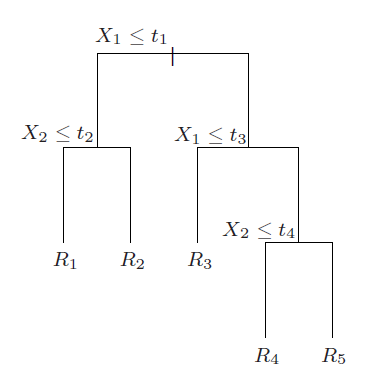
\includegraphics[width=0.4\textwidth]{Documentos Extra/Imagenes/Diagrama de arbol.png}}
 \caption{Representación de la división de $\mathbb{R}^p$ y el diagrama de árbol resultante}
 \label{f:MARC1}
\end{figure}


\subsection{Árboles de Regresión}

\subsection{Árboles de Clasificación }